\documentclass[journal,twoside,web]{ieeecolor}
% \documentclass[12pt,peerreview,draftversion,onecolumn,print]{ieeecolor}
\usepackage[table,x11names,svgnames,dvipsnames]{xcolor}
\usepackage[export]{adjustbox}
% \usepackage{algorithm}
% \usepackage[noend]{algpseudocode}
\usepackage{amsmath,amssymb,amsfonts}
\usepackage[USenglish]{babel}
\usepackage{bigints}
\usepackage{bm}
\usepackage{booktabs}
\usepackage{cancel}
\usepackage[tableposition=above, font=normalsize]{caption}
% \usepackage{centernot}
% \usepackage{comment}
\usepackage{empheq}
\newcommand*\widefbox[1]{\fbox{\hspace{2em}#1\hspace{2em}}}
\usepackage{enumitem}
\usepackage{epsfig}
\usepackage{epstopdf}
% \epstopdfsetup{outdir=./figures//}
% \usepackage[letterpaper, top=1.0in, bottom=1.0in, left=1.0in, right=1.0in]{geometry}
\RequirePackage[OT1]{fontenc}
% \usepackage{fontspec}
\usepackage{graphics}
\usepackage{graphicx}
\graphicspath{{../figures/}}
% \usepackage{ifpdf}
% \usepackage{lastpage}
% \usepackage{leftidx}
\usepackage{lineno}
\usepackage{lipsum}
% \usepackage{mathrsfs}
\usepackage{mathtools}
\usepackage{multicol}
\usepackage{multirow}
\usepackage{nicefrac}
% \usepackage{nicematrix}
% \usepackage{pgfplots}
\usepackage{pifont}
% \usepackage{ragged2e}
% \usepackage{rotating}
% \usepackage{stmaryrd}
\usepackage{siunitx}
\usepackage{soul}
\usepackage[caption=false]{subfig}
\usepackage{tabularx}
\usepackage{threeparttable}
\usepackage{tikz}
% \usepackage{tkz-euclide}
% \usepackage{ctable}
% \usetikzlibrary{matrix, arrows}
\usetikzlibrary{shapes.geometric, arrows, decorations.markings, shapes.arrows}

\newcommand{\minitab}[2][l]{\begin{tabular}{#1}#2\end{tabular}}

%%%%%%% TODO NOTES 
\usepackage{todonotes}
\setlength{\marginparwidth}{1.3cm}
\setlength{\marginparsep}{0cm}
\newcommand{\ctodo}[1]{\todo[size=\tiny]{#1}}
\newcommand{\nnparam}{\theta}
\newcommand{\pinn}{\pi_{\nnparams}}

\usepackage{ulem}
\usepackage{wrapfig}

\tikzstyle{startstop} = [rectangle, rounded corners, minimum width=1cm, minimum
height = 0.5cm, text centered, draw=black, fill=red!30]
\tikzstyle{io} = [trapezium, trapezium left angle=70, trapezium right angle=110,
minimum height=1cm, text width=3cm, text centered, draw=black, fill=blue!30]
\tikzstyle{process} = [rectangle, minimum width=2cm, minimum height=0.8cm, text
centered, text width=2cm, draw=black, fill=orange!30]
\tikzstyle{decision} = [diamond, aspect=1.25, minimum width=2cm, minimum height=0.5cm, 
text centered, text width=3cm, draw=black, fill=green!30]
\tikzstyle{arrow} = [thick, ->, >=stealth]




\makeatletter
\newcommand{\rmnum}[1]{\romannumeral #1}
\newcommand{\Rmnum}[1]{\expandafter\@slowromancap\romannumeral #1@}
\makeatother

\DeclarePairedDelimiter\ceil{\lceil}{\rceil}
\DeclarePairedDelimiter\floor{\lfloor}{\rfloor}

\newcommand{\bmat}[1]{\begin{bmatrix}#1\end{bmatrix}}
\newcommand{\pmat}[1]{\begin{pmatrix}#1\end{pmatrix}}
\newcommand{\ubar}[1]{\text{\b{$#1$}}}
\newcommand{\norm}[2]{\|{#1}\|_{{}_{#2}}}
\newcommand{\abs}[1]{\left|{#1}\right|}
\newcommand{\mbf}[1]{\mathbf{#1}}
\newcommand{\mc}[1]{\mathcal{#1}}
\newcommand{\dd}{\operatorname{d}\!}
\newcommand{\muc}[2]{\multicolumn{#1}{c}{#2}}
\newcommand*\Eval[3]{\left.#1\right\rvert_{#2}^{#3}}
\newcommand{\inner}[1]{\left\langle#1\right\rangle}
\newcommand{\pd}[2]{\frac{\partial #1}{\partial #2}}
\newcommand{\pdd}[2]{\frac{\partial^2 #1}{\partial #2^2}}
\newcommand{\el}[2]{\frac{\dd}{\dd t}\pd{\mc{L}}{\dot{#1}} - \pd{\mc{L}}{#1} = #2}
\newcommand{\elk}[2]{\frac{\dd}{\dd t}\pd{\mc{L}}{\dot{#1}_k} - \pd{\mc{L}}{#1_k} = #2_k}
\newcommand{\vectornorm}[1]{\left|\left|#1\right|\right|}
\newcommand{\dom}[1]{\textrm{dom}\;#1}
\newcommand{\bx}{{\bf x}}
\newcommand{\bu}{{\bf u}}
\newcommand{\cmark}{\ding{51}}%
\newcommand{\xmark}{\ding{55}}%
\newcommand*{\vertbar}{\rule[-1ex]{0.5pt}{2.5ex}}
\newcommand*{\horzbar}{\rule[.5ex]{2.5ex}{0.5pt}}

\newcommand{\idapbc}{\textsc{IdaPbc}}
\newcommand{\electric}{{\textcolor{blue}{\hspace{-0.5mm}$\bm{E}$\;}}}
\newcommand{\magnetic}{{\textcolor{red}{\hspace{-0.5mm}$\bm{B}$\;}}}

% \theoremstyle{plain}
% \newtheorem{thm}{Theorem}[section]
\newtheorem{thm}{Theorem}
% \makeatletter
% \@addtoreset{thm}{section}
% \makeatother
% \newtheorem{cor}[thm]{Corollary}
\newtheorem{lem}{Lemma}
% \newtheorem{claim}[thm]{Claim}
% \newtheorem{axiom}[thm]{Axiom}
% \newtheorem{conj}[thm]{Conjecture}
% \newtheorem{fact}[thm]{Fact}
% \newtheorem{hypo}[thm]{Hypothesis}
% \newtheorem{assum}[thm]{Assumption}
\newtheorem{prop}{Proposition}
% \newtheorem{crit}[thm]{Criterion}
% \theoremstyle{definition}
\newtheorem{defn}[thm]{Definition}
% \newtheorem{exmp}[thm]{Example}
\newtheorem{rem}{Remark}
% \newtheorem{prin}[thm]{Principle}

\DeclareMathOperator{\Tr}{tr}
\newcommand\xdownarrow[1][2ex]{%
   \mathrel{\rotatebox{90}{$\xleftarrow{\rule{#1}{0pt}}$}}
}
\DeclareMathOperator{\End}{End}
\DeclareMathOperator{\Hom}{Hom}
\DeclareMathOperator{\id}{id}
\DeclareMathOperator{\vers}{vers}
\DeclareMathOperator{\trans}{Trans}
\DeclareMathOperator{\rot}{Rot}
\DeclareMathOperator{\rank}{rank}
\DeclareMathOperator{\sinc}{sinc}

\usepackage{hyperref}
\hypersetup{
    unicode=false,          % non-Latin characters in Acrobat’s bookmarks
    pdftoolbar=true,        % show Acrobat’s toolbar?
    pdfmenubar=true,        % show Acrobat’s menu?
    pdffitwindow=false,     % window fit to page when opened
    pdfstartview={FitH},    % fits the width of the page to the window
    pdftitle={Mischievous Sibling's Grid World},    % title
    pdfauthor={Aykut C. Satici}, % author
    % pdfsubject={Subject},   % subject of the document
    % pdfcreator={Creator},   % creator of the document
    % pdfproducer={Producer}, % producer of the document
    % pdfkeywords={keyword1, key2, key3}, % list of keywords
    pdfnewwindow=true,      % links in new PDF window
    colorlinks=true,       % false: boxed links; true: colored links
    linkcolor=blue!30!green,          % color of internal links (change box color with linkbordercolor)
    linkbordercolor=orange,
    citecolor=blue,        % color of links to bibliography
    citebordercolor=green,
    filecolor=magenta,      % color of file links
    urlcolor=cyan,           % color of external links
    urlbordercolor=blue,
}

\usepackage{generic}

% Not sure if needed
\def\BibTeX{{\rm B\kern-.05em{\sc i\kern-.025em b}\kern-.08em
    T\kern-.1667em\lower.7ex\hbox{E}\kern-.125emX}}

\markboth{\journalname, VOL. XX, NO. XX, September 2022}
{Shortest Path on a Regular Pyramid}

\begin{document}

\title{Shortest Path on a Regular Pyramid} 
\author{
%     Wankun Sirichotiyakul, \IEEEmembership{Student Member, IEEE};
%     Nardos Ayele Ashenafi, \IEEEmembership{Student Member, IEEE};\\%
    Aykut C. Satici, \IEEEmembership{Member, IEEE}
%     \thanks{Submitted for review on 6 April 2022.}
%     \thanks{W. Sirichotiyakul and N. A. Ashenafi are with the Electrical and Computer Engineering Department, Boise State University, Boise, ID 83706 USA
%     (e-mail: \{wankunsirichotiyakul,nardosashenafi\}@boisestate.edu).}
    \thanks{A. C. Satici is with the Mechanical and Biomedical Engineering Department, Boise State University, Boise, ID 83706 USA
    (e-mail: aykutsatici@boisestate.edu).}
}
\maketitle
% \IEEEpeerreviewmaketitle

  
\begin{abstract} % Abstract of not more than 200 words.

This problem, seen on Mind Your Decisions channel~\cite{mindyourdecisions} on
YouTube, concerns finding the shortest distance to a particular point on a
regular pyramid, starting from a particular vertex.

\end{abstract}

\begin{IEEEkeywords}
  Geometry, Ti\textit{k}Z
\end{IEEEkeywords}

\section{Introduction}
\label{sec:intro}
%
The question is interesting and the solutions are just as interesting. Let us 
delve right into it.
\section{Problem Statement}
\label{sec:statement}

In addition to the problem statement given in the caption of
Figure~\ref{fig:problem}, we will also seek to find the path that yields the
shortest distance from the vertex $P$ to the point $T$, which lies in the middle
of the vertices $O$ and $R$.

\begin{figure}[h]
  \centering
  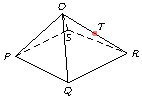
\includegraphics[trim={0 0 0 0cm},clip,width=0.5\textwidth]{./figures/pyramid.pdf}
  \vspace{-8mm}
  \caption{Shown above is a regular square pyramid all of whose sides have
  length of $2\ell$. We seek to find the shortest distance from the vertex $P$
  to the midpoint $T$ of points $O$ and $R$.}
  \label{fig:problem}
\end{figure}

% \begin{enumerate}
%   \setlength\itemsep{0em}
%   \item Find the map $f: \mathbb{R}_+^2 \rightarrow \mathbb{R}_+^2$ that takes
%           the side lengths of the rectangle $(w,h)$ to $(r, \abs{XY})$, the
%           radius of one of the circles and the length of the line segment $XY$.
%   \item Find the inverse $f^{-1}$ of $f$, that takes $(r, \abs{XY})$ to $(w,h)$.
% \end{enumerate}


\section{Problem Solution}
\label{sec:solution}

Shown in Figure~\ref{fig:unfolded}, we show the regular pyramid of
Figure~\ref{fig:problem} unfolded in a particular manner.

\begin{figure}[h]
  \centering
  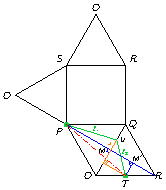
\includegraphics[trim={0 0 0
  0cm},clip,width=0.5\textwidth]{./figures/pyramid-unfolded.pdf}
  \vspace{-8mm}
  \caption{The regular pyramid unfolded.}
  \label{fig:unfolded}
\end{figure}


\section{Conclusion}
\label{sec:conclusion}

This is an interesting little brain teaser and a good excuse to practice some
more Ti\textit{k}Z.


\bibliographystyle{ieeetr}        
\bibliography{bib/pentahedron.bib}  

% \appendix

\newcommand*{\bbU}{\mathbb{U}}

\subsection{Computing the angle $\theta$ and $r$ from it}

The right triangle $\triangle CAD$ provides the equality \[ \tan{2\theta} =
\frac{2\tan{\theta}}{1-\tan^2{\theta}} = \frac{w}{h}, \] which implies the
quadratic equation \[ \tan^2{\theta} + 2\nicefrac{h}{w}\tan{\theta} - 1 = 0. \]
Solving for $\tan{\theta}$ such that $0 < \theta < \nicefrac{\pi}{2}$, we obtain
\[ \frac{r}{h-r} = \tan{\theta} = \nicefrac{1}{w}(d-h), \] where the first 
equality follows from the right triangle $\triangle EAX$. We can solve this
equation for the radius, $r$, which provides the solution
%
\begin{equation}
  r = \frac{h(d-h)}{w+d-h}.
  \label{eq:radiusalt}
\end{equation}
%
Simple computation shows that 
\[ \frac{h(d-h)}{w+d-h} = \nicefrac{1}{2}(w+h-d). \]


\end{document}
